\newpage
\section{SYSTEM DEVELOPMENT}
\subsection{Use Case Diagram}
\begin{figure}[h!]
        \centering
        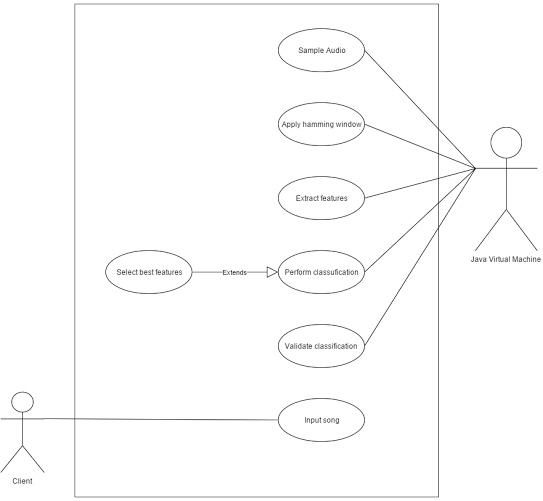
\includegraphics[width=150mm]{resources/mehang/softwaredevelopment/Usecase/usecase}
        \caption{Use case diagram}
\end{figure}
\newpage
\subsection{Data Flow Diagram}
\subsubsection{Level Zero}
\begin{figure}[h!]
        \centering
        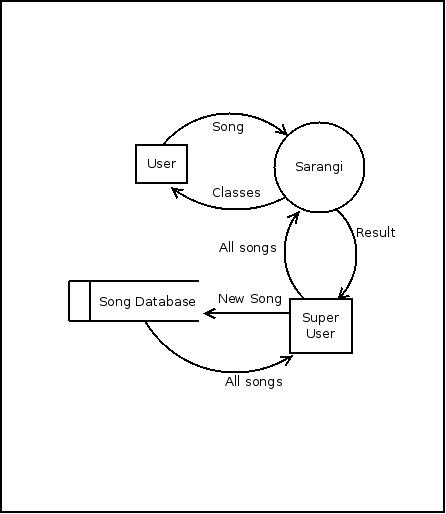
\includegraphics[width=110mm]{resources/mehang/softwaredevelopment/DFD/levelzero}
        \caption{Context level zero}
        \label{fig:contextlevel}
\end{figure}
\newpage
\subsubsection{Level One}
\begin{figure}[h!]
        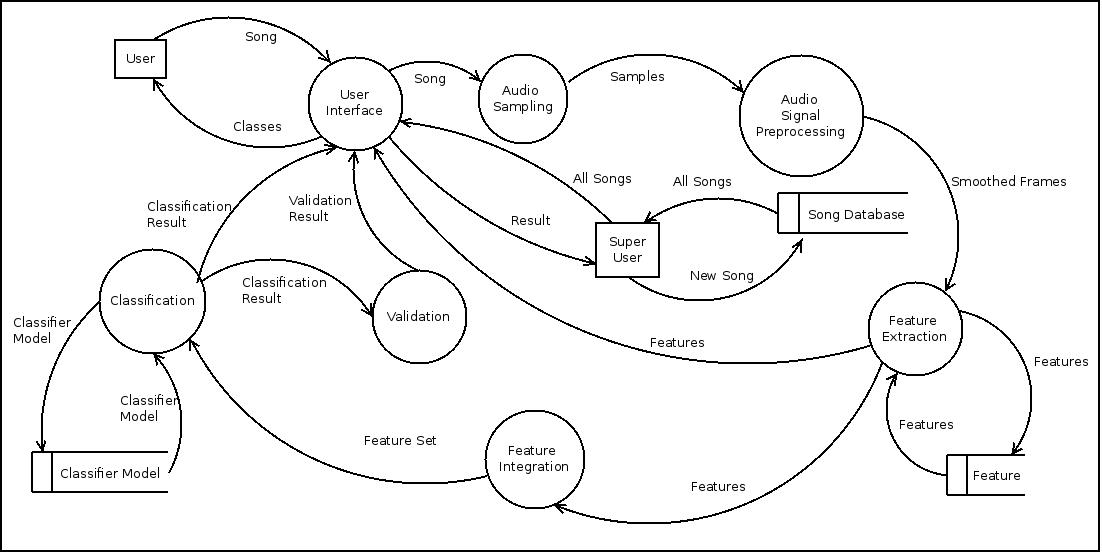
\includegraphics[width=170mm]{resources/mehang/softwaredevelopment/DFD/levelone}
        \caption{Context level one}
        \label{fig:level1b}
\end{figure}
\subsubsection{Level Two}
\vspace{20mm}
\begin{figure}[h!]
        \centering
        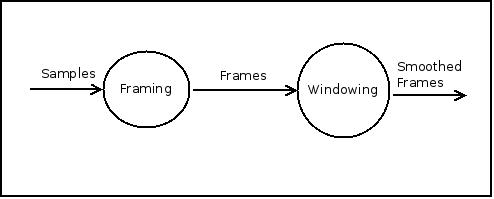
\includegraphics[width=100mm]{resources/mehang/softwaredevelopment/DFD/level2(audiosignalpreprocessing)}
        \caption{Audio signal pre-processing}
        \label{fig:pre-processing}
\end{figure}
\vspace{20mm}
\begin{figure}[h!]
        \centering
        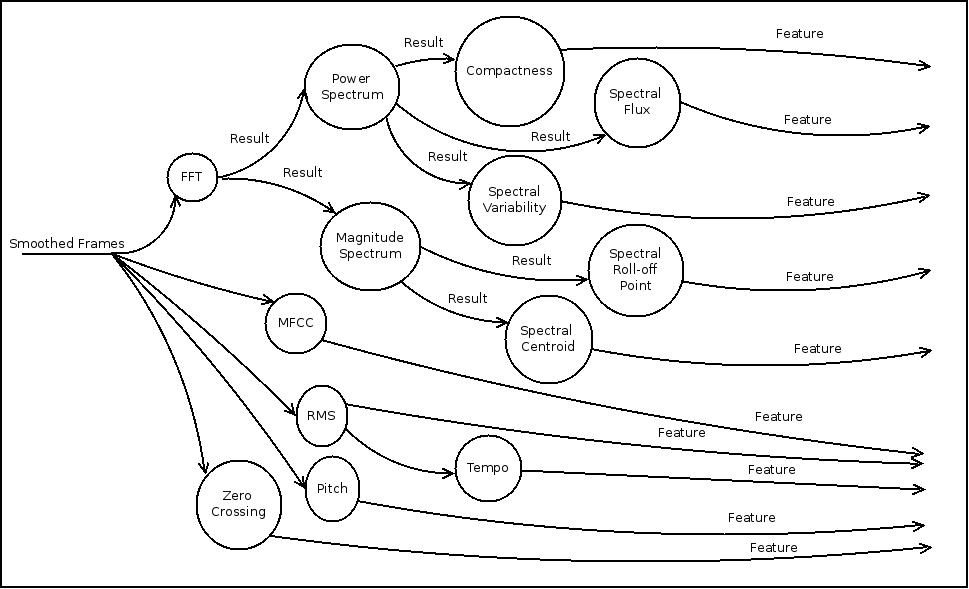
\includegraphics[width=170mm]{resources/mehang/softwaredevelopment/DFD/level2(featureextraction)}
        \caption{Feature extraction}
\end{figure}
\vspace{90mm}
\begin{figure}[h!]
        \centering
        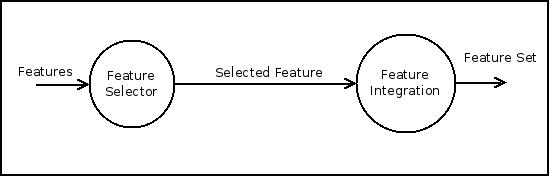
\includegraphics[width=150mm]{resources/mehang/softwaredevelopment/DFD/level2(featureintegration)}
        \caption{Feature integration}
\end{figure}
\vspace{90mm}
\begin{figure}[h!]
        \centering
        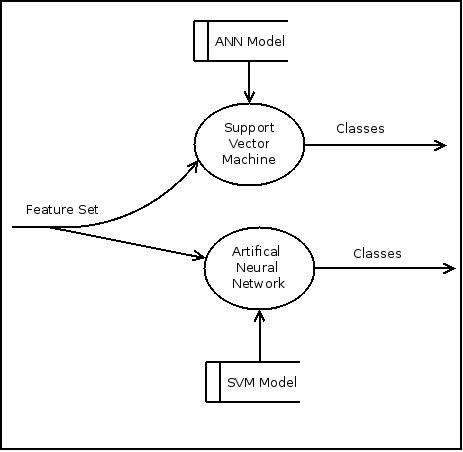
\includegraphics[width=80mm]{resources/mehang/softwaredevelopment/DFD/level2(classification)}
        \caption{Classifier}
        \label{fig:classifier}
\end{figure}
\vspace{50mm}
\begin{figure}[h!]
        \centering
        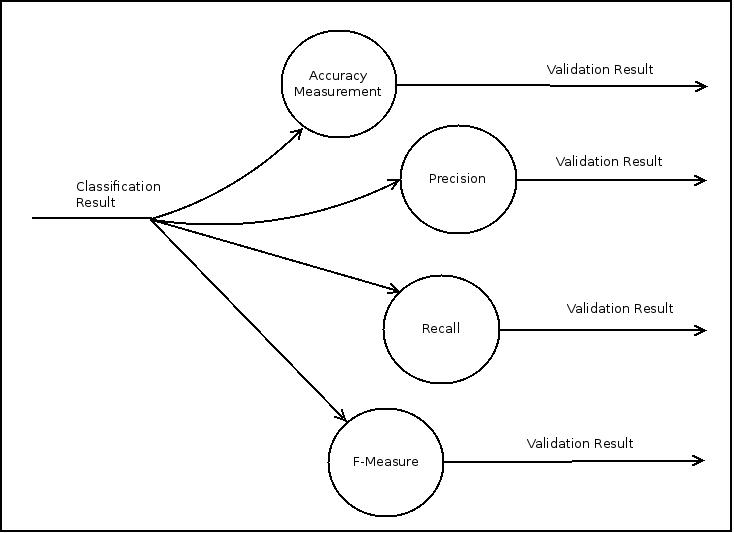
\includegraphics[width=110mm]{resources/mehang/softwaredevelopment/DFD/level2(validation)}
        \caption{Validation}
        \label{fig:validation}
\end{figure}
\newpage
\newpage
\subsection{Sequence Diagram}
\subsubsection{Feature Extraction}
\begin{figure}[h!]
        \centering
        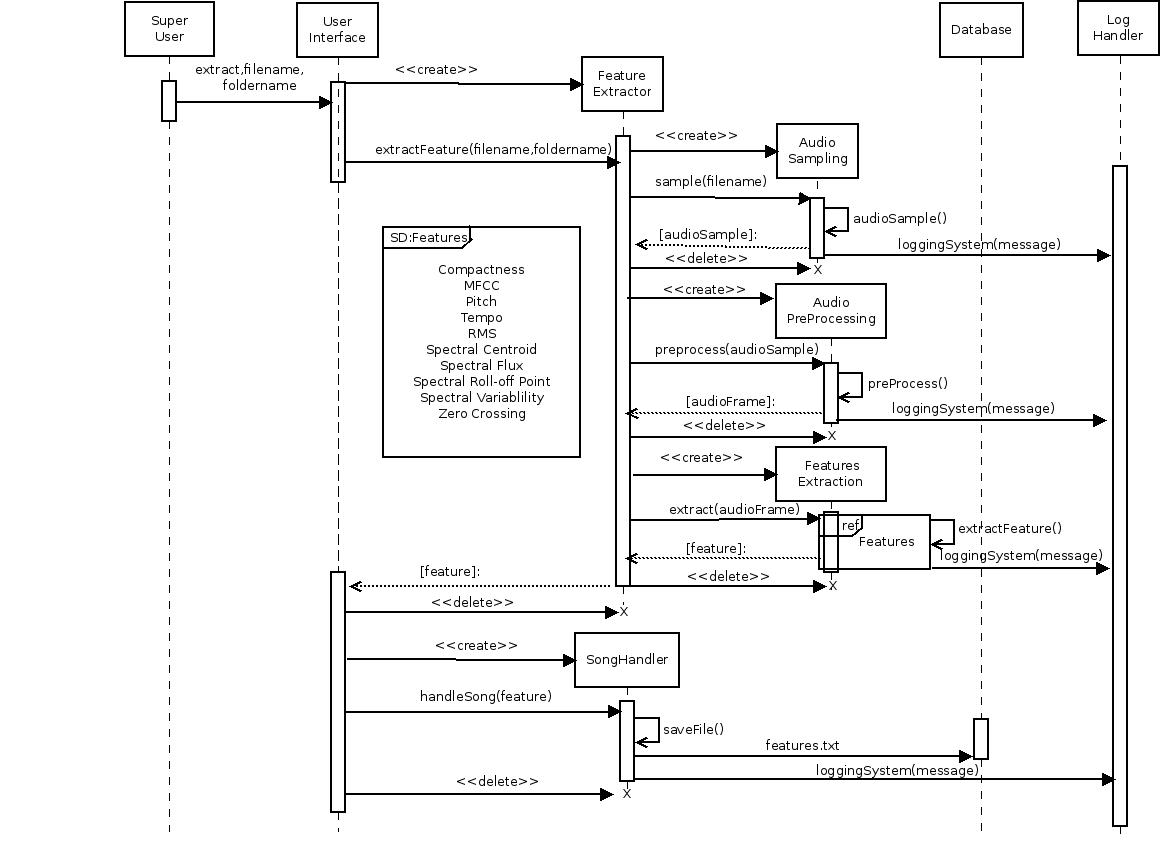
\includegraphics[width=160mm]{resources/sequence_featureextraction}
        \caption{Sequence diagram of extracting feature}
        \label{fig:sequence_featureextraction}
\end{figure}
\newpage
\subsubsection{Classification}
\begin{figure}[h!]
        \centering
        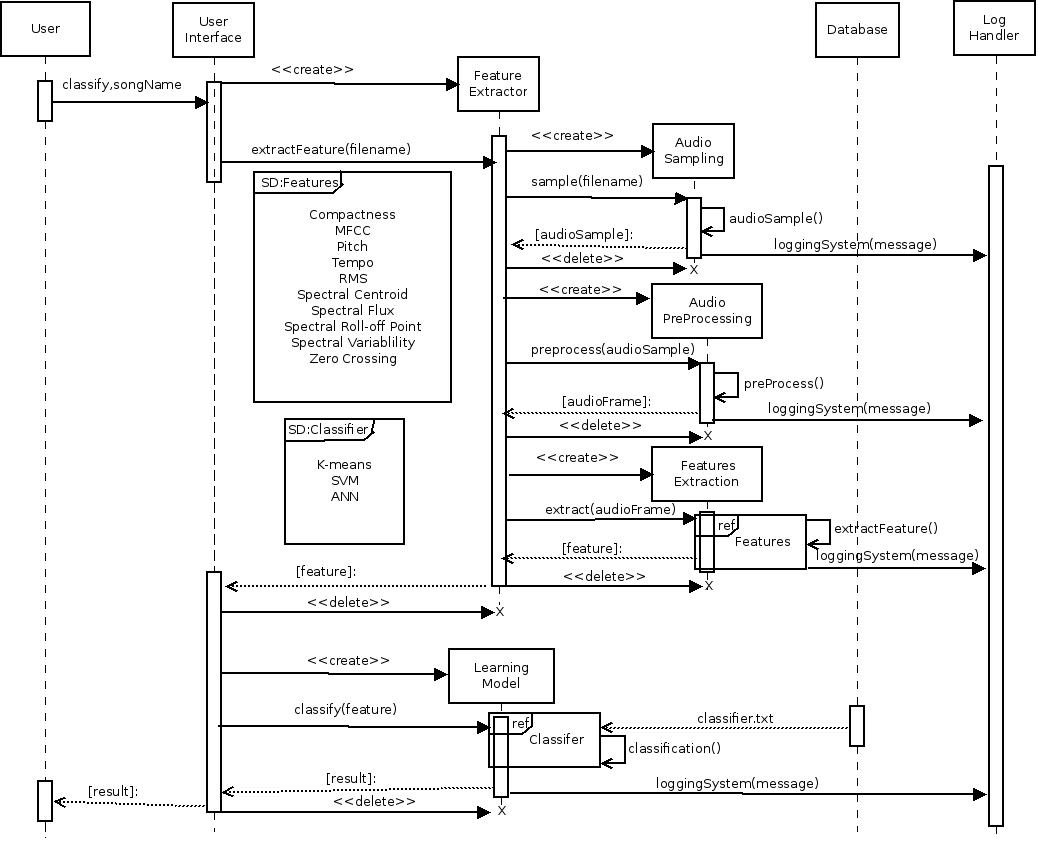
\includegraphics[width=160mm]{resources/sequence_classify}
        \caption{Sequence diagram of classification}
        \label{fig:sequence_classify}
\end{figure}
\newpage
\subsubsection{Training}
\begin{figure}[h!]
        \centering
        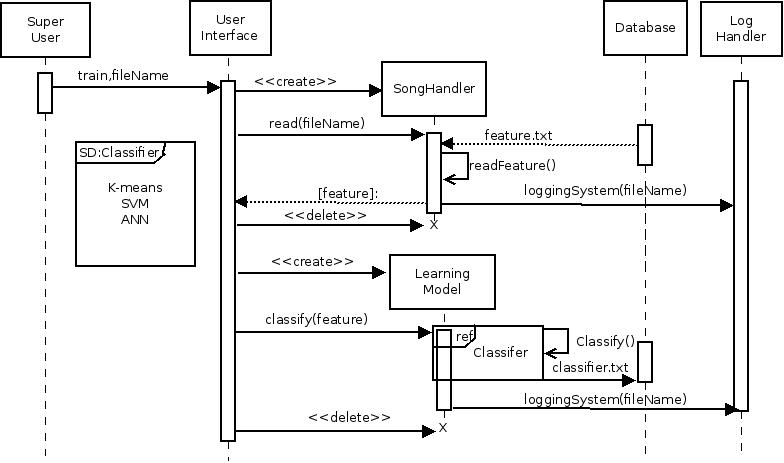
\includegraphics[width=170mm]{resources/sequence_training}
        \caption{Sequence diagram of training}
        \label{fig:sequence_training}
\end{figure}
\newpage
\newpage
\subsubsection{Testing}
\begin{figure}[h!]
        \centering
        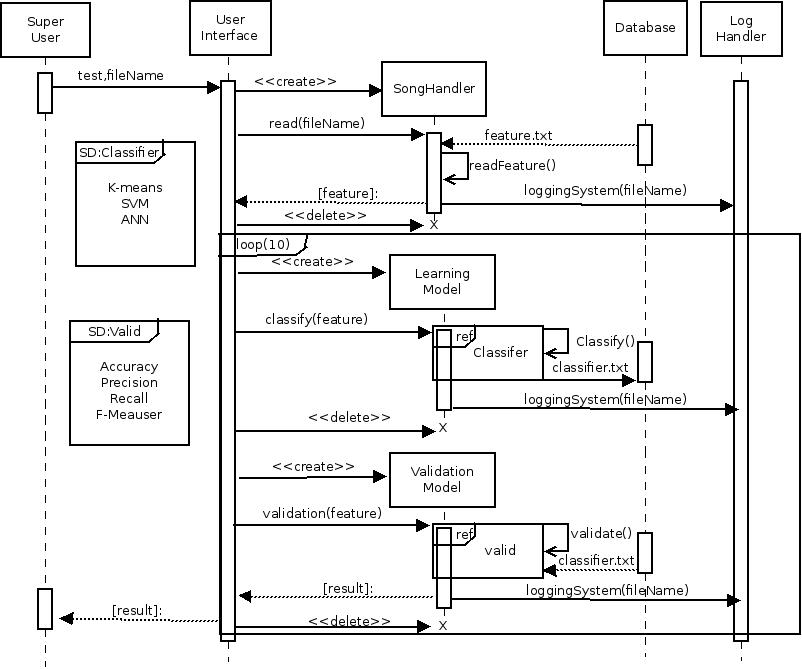
\includegraphics[width=160mm]{resources/sequence_test}
        \caption{Sequence diagram of testing}
        \label{fig:sequence_test}
\end{figure}


\subsection{Tools and Environment}

\subsubsection{Java Programming Language}

Java is a general-purpose computer programming language that is concurrent class-based, object-oriented. 
Java language is used for overall development of the system.
We chose java due to many reasons:

\begin{itemize}
    \item We were familiar with Java having worked on pretty decent sized Java projects.
    \item Although Java may be too verbose for small applications, we believe it is 
    \item Portability - Java runs well on all the popular platforms.
    \item Speed - The latest JIT compilers for Suns JVM approach the speed of C/C++ code, and in some memory allocation intensive circumstances, exceed it.
    \item Standard APIs that encompass lots of common funcionalities.
    \item GarbageCollection - the programmer doesn't have to worry about memory (most of the time).
    \item Availability of lots of Libraries, tools and frameworks in Java.
\end{itemize}

\subsubsection{SMILE - Statistical Machine Intelligence and Learning Engine}

SMILE (Statistical Machine Intelligence and Learning Engine) is a fast and comprehensive machine learning system. With advanced data structures and algorithms, Smile delivers state-of-art performance.
A stable released version of SMILE 1.1.0 is used for implement of complex machine learning algorithm like SVM,etc.
As mentioned in its documentation:
"Smile covers every aspect of machine learning, including classification, regression, clustering, association rule mining, feature selection, manifold learning, multidimensional scaling, genetic algorithms, missing value imputation, efficient nearest neighbor search, etc."

\subsubsection{TarsosDSP}

    TarsosDSP is a Java library used for audio processing. 
    Its aim is to provide an easy-to-use interface to practical music processing algorithms implemented, as simply as possible, in pure Java and without any other external dependencies. 
    The library tries to hit the sweet spot between being capable enough to get real tasks done but compact and simple enough to serve as a demonstration on how DSP algorithms works.
    We used TarsosDSP to process the low level song features.

\subsubsection{Google Gson}

Gson is a Java library that can be used to convert Java Objects into their JSON representation. 
It can also be used to convert a JSON string to an equivalent Java object. 
Gson can work with arbitrary Java objects including pre-existing objects that you do not have source-code of.  
We used Gson to store the features as JSON and read them back. 
We chose JSON because it is easily readable through a lot of methods, libraries and languages.

\subsubsection{Xstream}

XStream is a simple library used to serialize objects to XML and back again.
We used XStream to store the model as a XML file so that it can be read back. 

\subsubsection{MP3SPI}
MP3SPI is a Java Service Provider Interface that adds MP3 (MPEG 1/2/2.5 Layer 1/2/3) audio format support for Java Platform.
We used it to add a more reliable support for mp3 files.

\subsubsection{Python Programming Language}

Python is a high-level, general-purpose, interpreted, dynamic programming language.
We used Python scripts to handle the audio files and modify them to create the mood based dataset.

